\section{Motivation}

\begin{frame}{Why Hyperscan?}
  \begin{itemize}
    \item Modern algorithms cannot be fully understood by classical textbook techniques alone.
    \item In particular, modern regular expression engines are not just automata evaluators.
    \item Hyperscan combines graph decompositions, SIMD literal matchers (filtering and verification), and regular expression verifiers.
    \item This gives a productive source of theoretical questions theoretical questions.
  \end{itemize}
\end{frame}

\begin{frame}{From an Engine to a Statistic}
  \begin{center}
    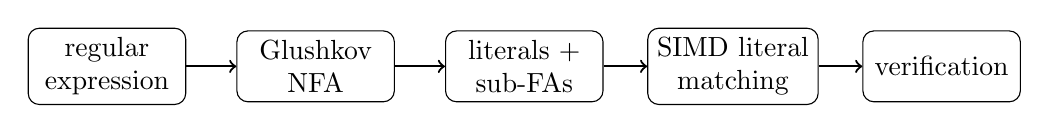
\begin{tikzpicture}[
        node/.style={draw, rounded corners, align=center, minimum width=2cm, minimum height=0.9cm},
        arrow/.style={->, thick}
      ]
      \node[node] (regex) at (0,0) {regular\\expression};
      \node[node] (nfa) at (2.65,0) {Glushkov\\NFA};
      \node[node] (split) at (5.30,0) {literals +\\sub-FAs};
      \node[node] (scan) at (7.95,0) {SIMD literal\\matching};
      \node[node] (verify) at (10.60,0) {verification};

      \draw[arrow] (regex) -- (nfa);
      \draw[arrow] (nfa) -- (split);
      \draw[arrow] (split) -- (scan);
      \draw[arrow] (scan) -- (verify);
    \end{tikzpicture}
  \end{center}

  \vspace{0.35cm}

  \textbf{Example:} For
  \texttt{ab[0-9]}\textsuperscript{\texttt{*}}\texttt{xy},
  Hyperscan finds positions of \texttt{ab} and \texttt{xy},
  then verifies the middle part with
  \texttt{[0-9]}\textsuperscript{\texttt{*}}.

  \textbf{Guiding idea:} Extracted literals are implementation details. Their lengths are a part that influences how selective the SIMD filtering phase is.
\end{frame}
